\subsection{Spectra}\label{sec:spectra}
%schriste - this section needs major work
%ji - there is no example of a spectrum

%ayshih - this whole paragraph can be deleted
%ji - I agree, this is redundant in such a journal.
Spectroscopy is the study of radiative energy as a function of wavelength.
An spectrum is normally obtained by observing a range of frequencies at the same time; 
it can be measured for example in radio wavelengths by a frequency sweep with 
a radio receiver or in visible and ultraviolet by the dispersion of the incident light 
through a diffraction grating or prism.
The analysis of the resultant spectrum can provide properties of the plasma observed 
such temperature, density, speed, etc.
Therefore, spectroscopy provides to the solar physicists invaluable information about 
the composition and the physical properties of the Sun.  

SunPy aims to provide broad support for solar spectroscopy
instruments.  The variety and complexity of these instruments and
their resultant datasets makes it very challenging to support all in a
general way.  The \texttt{spectra} module implements a
\texttt{Spectrum} class for 1D data (intensity versus frequency) and a
\texttt{Spectrogram} class for 2D data (intensity versus time and
frequency).  Each of these classes use a \texttt{numpy.ndarray} class
as its \texttt{.data} attribute.  These two classes were implemented
by funding provided by the Astrophysics Research Group at Trinity
College Dublin, Ireland.

The \texttt{Spectrogram} class supports radio spectrograms from the e-Callisto 
solar radio spectrometer network (\url{http://www.e-callisto.org/})
and STEREO/SWAVES spectrograms.
As with other SunPy data types, the \texttt{Spectrogram} class has been
built so that each instrument initialises using a subclass containing the instrument-specific 
functionalities.
%The common functionality provided by the base \texttt{Spectrogram} class includes
%reading data,
%joining different time ranges and frequencies,
%performing frequency-dependent background subtraction,
%and convenient visualization and sampling of the data.

Listing \ref{code:spectra} shows how the \texttt{CallistoSpectrogram}
object retrieves spectrogram data in the time range specified taken at
the observatory of interest.  When the data is requested using the
\texttt{.from\_range} function, the object merges all the downloaded
files downloaded into a single spectrogram, across time and frequency.
In the example shown, data is observed in two frequency ranges, 
20--90\,MHz and 55--355\,MHz.  Since the data is not evenly spaced in
the frequency range, the \texttt{Spectrogram} object linearises the
frequency axis for a better analysis.  The example also demonstrates
the implemented background subtraction method.
%ji to DPS - what is the linearisation that is happening here?

\begin{listing}[H]
\begin{minted}[bgcolor=bg]{pycon}
>>> from sunpy.spectra.sources.callisto import CallistoSpectrogram
>>> tstart, tend = "2011-06-07T06:00:00", "2011-06-07T07:45:00"
>>> callisto = CallistoSpectrogram.from_range("BIR", tstart, tend)
>>> callisto_nobg = callisto.subtract_bg()
>>> callisto_nobg.peek(vmin = 0)
\end{minted}
\begin{center}
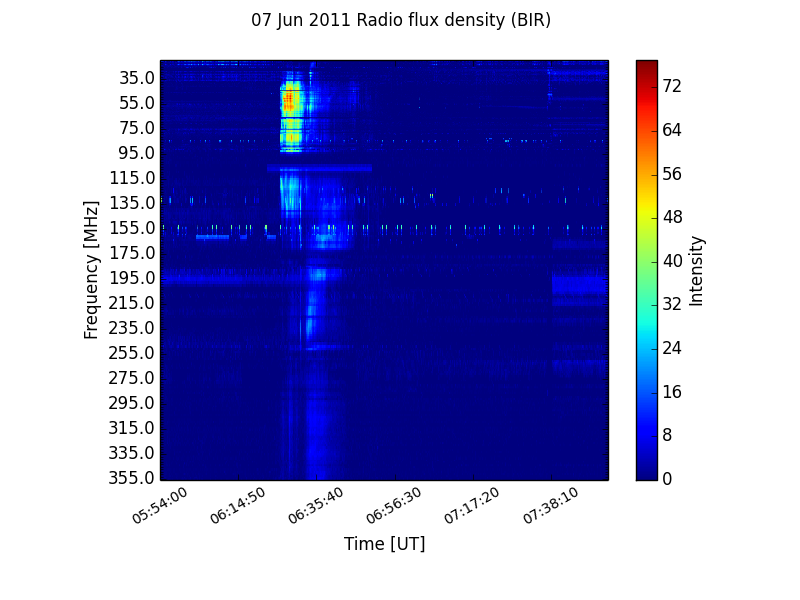
\includegraphics[width=0.8\columnwidth]{callisto_nobg}
\end{center}
\caption{Example of how \texttt{CallistoSpectrogram} retrieves the
  data for the requested time range and observatory, merges it and
  removes the background signal.  The data requested -- 'BIR' -- is
  the code name of the Rosse Observatory at Birr Castle in Ireland
  (\url{http://www.rosseobservatory.ie})}
\label{code:spectra}
\end{listing}

% Download Callisto
% Merge multiple time-ranges / frequencies (just work from downlad!)
% Merge callisto with swaves

